\documentclass{article}
\usepackage[utf8]{inputenc}
\usepackage{caption}
\usepackage[margin=1in]{geometry}
\usepackage{graphicx}
\graphicspath{ {Images/Assignment3} }
\usepackage{amsmath}
\usepackage{algorithm}
\usepackage[noend]{algpseudocode}


\title{Assignment 3: Random Forests}
\author{Lorenzo Meninato}
\date{April 2018}

\begin{document}

\maketitle

Given data collected on the features of coral reefs and their surroundings, I will develop a forecasting procedure to determine which coral reefs are at risk of reef bleaching. If reef bleaching is forecast for a given reef, I will recommend establishing a marine reserve at that location, which would prohibit all human activities, but research, at that given reef. Establishing a marine reserve would prevent locals from extracting resources from that marine area, so if a reef is incorrectly predicted to be at risk of bleaching, the local economy would unjustly suffer. On the other hand, if bleaching is correctly predicted, but no marine reserve is established, then a dying reef would provide little economic value to the area. Therefore, I will also need to specify an appropriate target cost ratio to balance possible asymmetric classification costs.

\section{Introduction}
Scientists have been monitoring coral reefs since the 1850s, but with the introduction of scuba diving in the 1960s, reefs were viewed and documented in a new fashion. In the 1980s scientists raised concerns about a decline in coral reef health at many well-researched reefs. Scientific discussions on coral reef health have been controversial. Some scientists argued that only a few reefs were at serious risk, while other reefs were only experiencing a temporary downturn. In response, scientists concluded that more data was needed to obtain a complete picture of the health of coral reefs around the world. Up until that point, a small number of reef scientists had been carrying out surveys using different methods at few locations. The solution became to organize a global survey effort using one standard method to gain a complete view of the health status of the world's reefs. The dataset this paper relies on begins in 1997, when scientists began volunteering as Reef Check Trainers to carry out a global survey of reef health across 31 countries. The immediate results of the survey suggested that, on a global scale, coral reefs were undergoing a health crisis. Since then, hundreds of Reef Check teams have been monitoring reefs on a yearly basis and more countries have began participating. This dataset contains data on the features of coral reefs and their surroundings from 1997 to 2017. I only consider data collected at the level of the reef, not the transect or diver. 

The dataset is fairly complete. There are 12392 observations over 12 variables from 1997 to 2017. While there are no missing observations, several of the variables had ``blank'' as a possible coding for the categorical variables, for instance, the Ocean, Human Impact, Siltation, Sewage, etc. variables. These variables usually also had a ``none'' ``never'' classification as well, so I combined the blank level with that level. So if the variable Poison had 3000 observations in the ``blank'' category and 6000 observations in the ``none'' category, I coded the variable as simply having a ``none'' category with 9000 observations. There is some concern in doing this. Mainly, if ``blank'' observations were erroneously placed into that category, then instead we would have wanted to impute the ``blank'' observations into the other categories at the frequency which they occurred. However, based on the methodology with which the Reef Check dataset was compiled, it seems likely that if a category did not apply, like if Poison was not present near the reef, then the recorder might have simply left the data point blank, whereas the more robust data entry action would have been to categorize the Reef's Poison variable as ``none''. I would argue that before commencing with Level I and or Level II analysis, it would be necessary to justify any undertaking with respect to how the ``blank'' category was handled across many of the variables, since thousands of observations were codified as ``blank''. A less severe problem was how to handle unknown or strange categories in the factor levels of the variables. There were much fewer observations of those types. For Ocean variable, I did not change the ``unknown'' factor level, but for the other variables I combined the ``unknown'' level with the ``none'' or ``never'' level. Similarly, I did not change the ``prior'' level in the Dynamite variable. The final data manipulation I performed was re-ordering the factor levels, where applicable. So for instance, in the ``Human Impact'' variable, it is more logical for the ordering of the factors to be ``none'' $\leq$ ``low'' $\leq$ ``moderate'' $\leq$ ``high'' rather than ``none'' $\leq$ ``high'' $\leq$ ``moderate'' $\leq$ ``low''. I performed a similar transformation where applicable. While the Random Forest algorithm might ignore the ordering of the factor variables, for the scalability of the dataset, and when comparing the Random Forest algorithm to other machine learning techniques, it seemed appropriate to have a consistent ordering of the factor variables.


\section{Univariate Analysis}

First, I begin with a cursory analysis of the variables in the dataset. Only about 3\% of the reefs experienced some form of bleaching, implying that there are only 361 instances of bleaching. This could diminish the statistical strength of the final forecasting model, since are fewer ways for the Random Forest algorithm\footnote{I give a general overview of how bagging and random forest algorithms work in the Random Forest section.} to select features that lead to a ``Yes'' prediction. 

\begin{figure}[!htb]
    \centering
    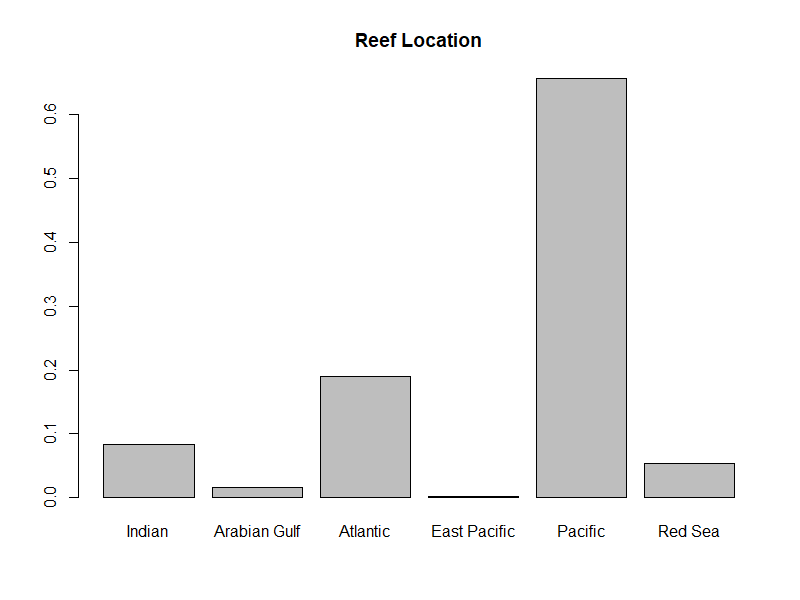
\includegraphics[scale=0.5]{/ocean.png}
    \caption{Density of reef location across oceans.}
    \label{ocean}
\end{figure}

The reefs appear to be primarily located in the Pacific ocean, with a significant amount of reefs in the Atlantic and Indian oceans. Later, I will compare the reef locations for bleached reefs versus healthy reefs. In Figure \ref{depth} I note that the depth of the reefs is clustered around 3-5 meters and around 10 meters. It will be interesting to see how the depth varies across bleached reefs and healthy reefs. Since I do not have a solid grasp of the underlying subject matter, I cannot make a strong prediction about how significant the impact of reef depth would have on a reef's susceptibility to bleaching. But, I would weakly conjecture that reefs that are shallower, say clustered around 3-5 meters rather than 10 meters, would be more vulnerable to commercial activity and other forms of human impact that occur around that depth. 

\begin{figure}[!htb]
    \centering
    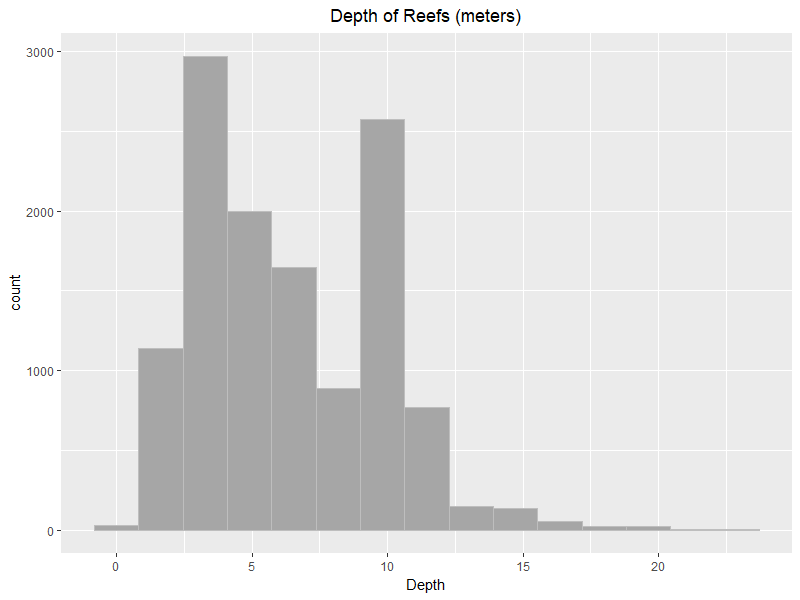
\includegraphics[scale=0.5]{/depth.png}
    \caption{Histogram of the depth of reef locations.}
    \label{depth}
\end{figure}

In Figure \ref{human} I record the relative frequencies at which each factor in the categorical variables for various forms of possible human impacts on the reefs. Overall, roughly 75\% of observations recorded some form of human impact. So it seems feasible that there is some form of a relationship between human activity and reef health. Siltation is not necessarily caused by humans, but its distribution is likely a function of the human impact on the transect near the reef. For instance, fertilizer run-off from agriculture could certainly affect the siltation levels. The siltation categorical variable would probably be more useful if it had been a numerical variable instead, since the distinction between the categories seems arbitrary, and in reality, it is likely the data is much more granular. The presence of poison appears to be quite low overall, so the sewage variable probably captures more of the effect of run-off from human activities. 

\begin{figure}[!htb]
    \centering
    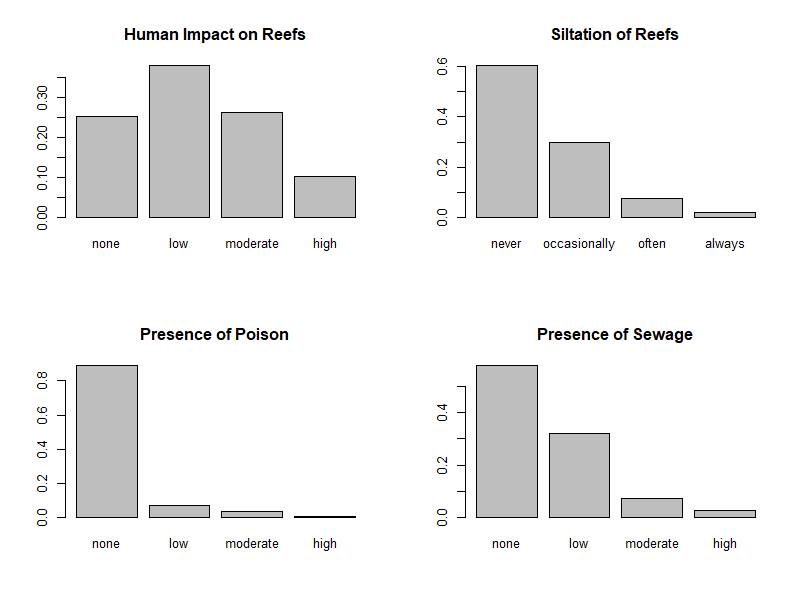
\includegraphics[scale=0.5]{/humanimpact1.png}
    \caption{Histograms of several human presence indicator variables.}
    \label{human}
\end{figure}

Lastly, I think before commencing a Level II analysis, it is crucial to make a statement on the quality of the data. The distribution of the years when data were collected, seen in Figure \ref{year}, varies greatly. From 1997 to the early 2000s, there was a great increase in observations, but from 2012 to 2017 it seems that data were collected less frequently. This is not necessarily a problem, but examining the bivariate relationships between the Years variable and the dependent variable, I feel it is necessary to raise a concern about the quality of the data. 

\begin{figure}[!htb]
    \centering
    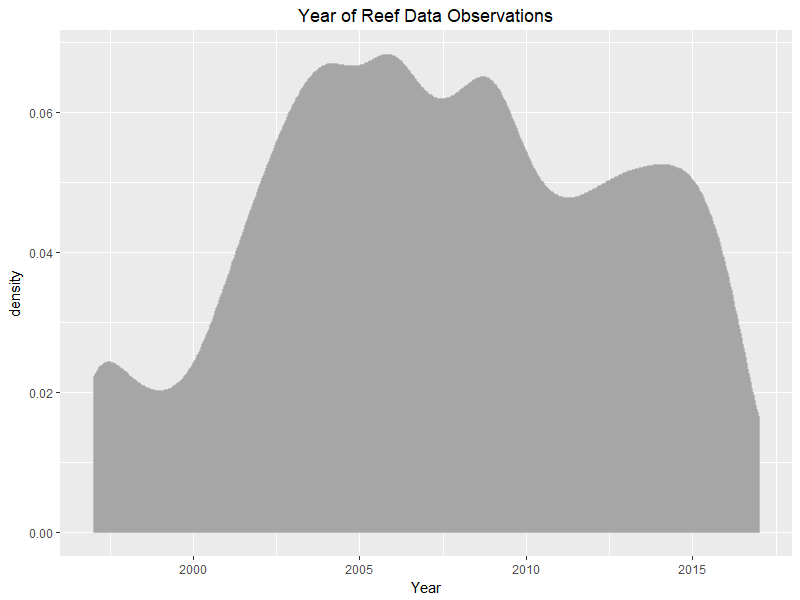
\includegraphics[scale=0.5]{/year.png}
    \caption{Year of Reef-Level Observation.}
    \label{year}
\end{figure}

\newpage

\section{Bivariate Analysis}
At the top of Figure \ref{yearB} we see that the data were collected as expected in Figure \ref{year}, but the bottom graph is concerning. All the observations of bleached reefs occurred in clusters around 1998 and 2002. There are $\textbf{no}$ observations of bleached reefs after 2003. This could have some serious implications about how the random forest algorithm will weight the importance of the year of the observation. For that reason, it could be interesting to examine how the algorithm is different if the year is omitted. In either case, this raises concerns about the quality of the data. Did the methodology for classification of reef health change after 2003? Are there missing observations of bleached reefs after 2003? It would be difficult to answer these questions with my current resources, therefore it makes my future forecasting model more tenuous. Regardless, even if the model will be flawed in certain ways, with a fuller understanding of the limitations of a ``flawed'' model, I can still discern useful information and implications from a flawed model. \\

\begin{figure}[!htb]
    \centering
    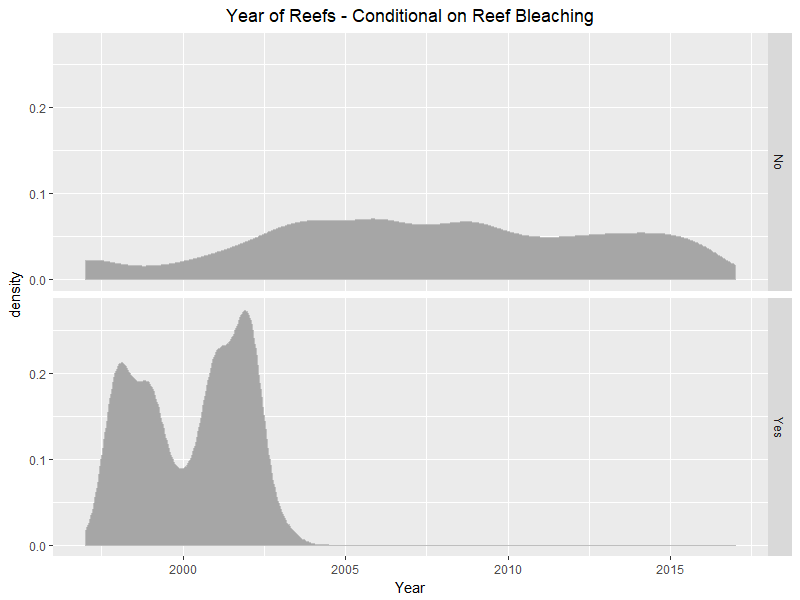
\includegraphics[scale=0.5]{/YearsBleaching.png}
    \caption{Year of Reef-Level Observation for Bleached and Healthy Reefs.}
    \label{yearB}
\end{figure}

A rough analysis of the location of bleached reefs shows that the Indian (5\% more likely) and Atlantic (1.2\% more likely) oceans are present at higher frequencies than the Pacific ocean\footnote{See Figure \ref{oceanB}}. \\

\newpage 

\begin{figure}[!htb]
    \centering
    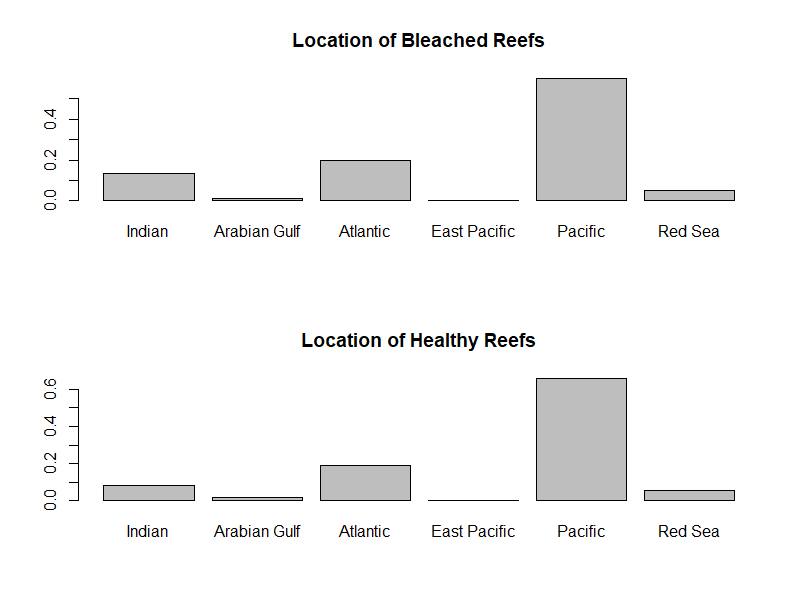
\includegraphics[scale=0.5]{/oceanB.png}
    \caption{Location of Bleached and Healthy Reefs}
    \label{oceanB}
\end{figure}

The conditional distributions of the depth of reefs, noted in Figure \ref{depthB}, appear to be almost identical for bleached and healthy reefs. The distribution of the bleached reefs is smoother, and appears to be slightly more right-skewed than the healthy reefs, which could support my earlier hypothesis that shallow reefs are at a higher risk of significant ecological change, as defined in the Reef Check manual on page 45\footnote{On page 45 the authors note that ``Many managers feel that a change of 50\% or more over a period of 1
year would be required to trigger management action.''}.\\

\begin{figure}[!htb]
    \centering
    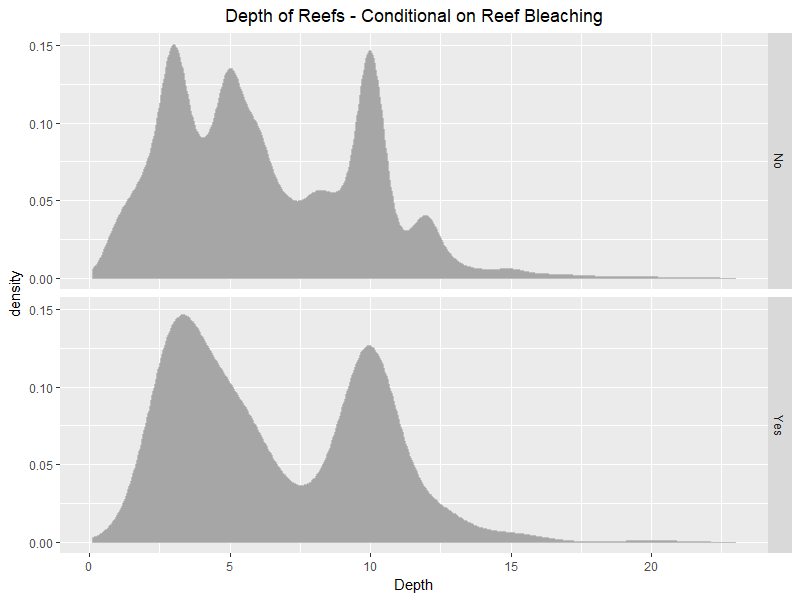
\includegraphics[scale=0.5]{/depthB.png}
    \caption{Depth of Reefs for Bleached and Healthy Reefs}
    \label{depthB}
\end{figure}

In Figure \ref{humanimpactB} I give an overview of the differences between instances of human activity across bleached and healthy reefs. While the storms variable had less impact than I might have guessed, there are several noteworthy results from this analysis. First, I note that the proportion of bleached reefs with no human impact is much lower than that of healthy reefs. Likewise, sewage presence has a similar correlation with the health of a reef. Interestingly, bleached reefs had very little presence of siltation. There might be an underlying subject-matter knowledge related effect that could explain this, but I would not be able to say anything strong about this result. The commerce variable conditional distribution is even more surprising. Almost all observations of bleached reefs had no presence of commercial activity \footnote{While I am a bit puzzled by some of these results, I do not think this is a mistake. My code is attached in the appendix.}. 

Of course, there could be many additive and non-linear interactions between the variables that are not captured by an initial univariate and bivariate analysis, so simply because there is nothing striking about a bivariate analysis, we cannot expect there to be no interaction between a variable and the dependent variable, especially considering how a variable could have complicated interactions with the roughly 10 other variables. 
\begin{figure}[!htb]
    \centering
    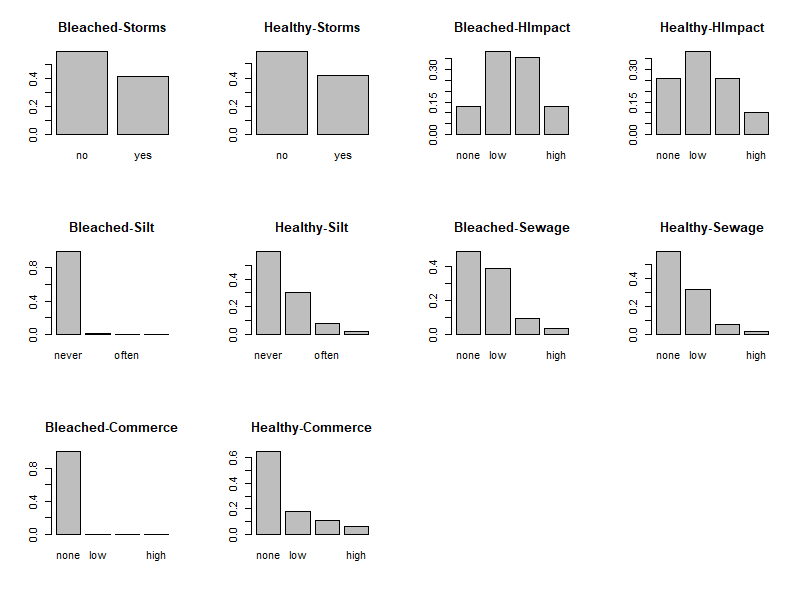
\includegraphics[scale=0.6]{/humanimpactB.png}
    \caption{Frequency of recorded human activity for Bleached and Healthy Reefs}
    \label{humanimpactB}
\end{figure}

The goal of a level II analysis is to produce an estimate of the true response surface that is as close as possible to the truth. This must be done with a judicious understanding of the bias-variance tradeoff. To justify a level II analysis, I must be confident to some degree that the estimation target is the approximate response surface, and therefore there is no biased, at least asymptotically. So are the fitted value of a statistical model estimates of the conditional expectations of the response surface approximation? I think it is more than reasonable to assume that the Reef Check data are derived from the true response surface, since the science discussed in the 2016 Reef Check instruction manual seems like a fair assessment of the correlates between reef health and various independent variables. With that assumption in mind, it is more than fair to proceed with a level II analysis. However, a biased approximation may emerge if there is reason to believe that the data is not sampled from the appropriate joint distributions. As I highlighted earlier, there is at least some weak evidence that perhaps the data is incomplete and or imputed improperly. Regardless, the core of the data seems fairly intact, thus if there are interesting and complex interactions between variables, an appropriate machine learning algorithm like a model ensemble algorithm may be able to tease out those interesting nonlinearities. 

\newpage

\section{Random Forests}

Before commencing with the implementation of the random forest algorithm, I must justify an appropriate cost ratio. There are two competing forces at play: the trade-off between having more false negatives versus having more false positives. False negatives, in this case, would be when the model forecasts that a reef would be healthy, when in fact the reef underwent some degree of bleaching. This would be concerning to the data analyst since resources could have been spent to protect that at-risk reef and instead the reef is not only lost, which provides an important ecological service to the nearby marine life, but also we would expect the local economy to suffer, since now less marine resources could be extracted from that area. The cost of false negatives, however, must be considered in tandem with the cost of false positives. False positives, in contrast, would be instances where the model predicts that reef will be at risk of bleaching, when in reality the reef was not risk. The cost of false positives, therefore is simply the cost of needlessly allocating resources to protecting the marine reserve. I do not have the relevant subject-matter knowledge to accurately assess which economic cost dominates the other. However, the research does suggest that once a reef undergoes bleaching, not only is the surrounding marine life adversely impacted, but it is both difficult and costly to help reefs recover from bleaching. Further, one way to quantify the economic value of a healthy reef is to consider the volume of greenhouse gases that could be sequestered by a healthy reef, and then adjust the cost ratio appropriately. For the reasons I have outlined, I think that it is more important for the model to avoid false negatives rather than false positives. The exact appropriate ratio is difficult to quantify, but roughly, I would argue that a false negative is three to five times more costly than a false positive. I made this rough estimating by weighing the fact that it is costly, both economically and ecologically, to have coral reef bleaching take place. It does not seem that expensive to unnecessarily protect a reef, therefore the cost of a false positive should be far lower than the cost of a false negative. To be conservative, I will choose a cost ratio of 5:1.
\newpage

\subsection{Model Ensemble Algorithms}
While it is not a complicated task to run the data into a statistical computing language into R, understanding how relevant statistical learning models work is key to understanding the tuning parameters and guides the data analyst as to how he or she should proceed with analyzing the results.
\begin{algorithm}
\caption{Bagging($D$, $T$, $\mathcal{A}$)- train an ensemble of models from bootstrap samples}\label{bagging}
\begin{algorithmic}[1]
\Procedure{Bagging}{}
\State $\text{Input: data set $D$; ensemble size $T$; learning algorithm $\mathcal{A}$}$
\For{t=1 \text{to} $T$ }
\State $\text{build a bootstrap sample $D_t$ from D by sampling $|D|$ data points with replacement}$
\State $\text{run $\mathcal{A}$ on $D_T$ to produce a model $M_t$}$
\EndFor
\State \Return $\{M_t | 1 \leq t \leq T\}$
\State $\text{Output: ensemble of models whose predictions are to be combined by voting or averaging}$
\EndProcedure
\end{algorithmic}
\end{algorithm}

We can see that the RandomForest algorithm is an ensemble of the bagging method. The idea is fairly simple: build each tree from a different random subset of the features. In general, increasing the number of iterations, or the ensemble size $T$, will improve results, but eventually the trade-off between computational intensity and out-of-bag (OOB) error is not worthwhile. In terms of handling asymmetric classification costs, of the four most common approaches to cost tuning, using stratified sampling will be demonstrably superior since the response variable is highly unbalanced (there are many more ``No'' results than ``Yes''). Note that this is because any given bootstrap sample may fail to have sufficient observations for the ``Yes'' category. 


\begin{algorithm}[!htb]
\caption{RandomForest($D$, $T$, $d$)- train an ensemble of tree models from bootstrap samples and random subspaces}\label{RandomForest}
\begin{algorithmic}[1]
\Procedure{RandomForest}{}
\State $\text{Input: data set $D$; ensemble size $T$; subspace dimension $d$}$
\For{t=1 \text{to} $T$}
\State $\text{build a bootstrap sample $D_t$ from D by sampling $|D|$ data points with replacement}$
\State $\text{select $d$ features at random and reduce dimensionality of $D_t$ accordingly}$
\State $\text{train a tree model $M_t$ on $D_t$ without pruning}$
\EndFor
\State \Return $\{M_t | 1 \leq t \leq T\}$
\State $\text{Output: ensemble of tree models whose predictions are to be combined by voting or averaging}$
\EndProcedure
\end{algorithmic}
\end{algorithm}

\subsection{Model Results}

For tuning the bootstrap samples I begin by considering the sample size for the less common category, ``Yes'', and compute two-thirds the number of times it occurs in my training set ($283$ times). So I know that the sample size of the less frequent outcome must be about $187$. From there I check various values for the other category, until I reach the target cost ratio\footnote{I found a cost ratio of 4.92 when I had the parameter $\textit{sampsize}= c(1150, 187)$.}. In Table 1, I note that the preliminary results are fairly good with an OOB error around 4.9\%. While OOB error estimates are useful, random forests are prone to over-fitting, thus it will be necessary to examine the confusion matrix when the model is fitted on the test dataset. 



\begin{table}[!htb]
\centering
\label{random1}
\begin{tabular}{|l|ll|ll|}
\hline
          & Classify as No Bleaching & Classify as Bleaching & Model error &  \\
          \hline
No Bleaching     & 9226               & 404             &  .04      &  \\
 Bleaching       & 82                 & 201             &  .29      &  \\
\hline
Use error        & 0.01               & 0.67            & 0.0497    &  \\
\hline
\end{tabular}
\caption{Confusion table for classifying risk of coral reef bleaching with 5:1 cost ratio.}
\end{table}

The following table is fairly strong evidence that the random forest was fairly useful for this forecasting problem. In particular, the distribution of model and use errors is very similar to the confusion table from the model using the training data. If this were not true, it would imply the response surface the model is attempting to estimate does not accurately reflect the true response surface. Hence, $\textit{if we assume}$ that the assumptions about the data being representative of the appropriate joint probability distributions, then this model will likely work fairly well as a forecast of which reefs will be at risk of bleaching. 

\begin{table}[!htb]
\centering
\label{predict}
\begin{tabular}{|l|ll|ll|}
\hline
          & Classify as no Bleaching & Classify as Bleaching & Model error &  \\
          \hline
No Bleaching     & 2296              & 105             &  .04      &  \\
 Bleaching       & 23                & 55              & .29       &  \\
\hline
Use error        & 0.01              & 0.65            & 0.052     &  \\
\hline
\end{tabular}
\caption{Confusion table for forecasts of coral reef bleaching with 5:1 cost ratio.}
\end{table}

\subsection{Importance of Predictors}

In Figure \ref{vip} we see how much prediction accuracy is reduced by when each predictor is randomly shuffled. However, this diagram does not show how an input is related to the response. From this plot we cannot say anything about the functional form of the relationship between the outcome variable and any of the predictors. Interestingly, randomly shuffling the commercial and the siltation variables increases the accuracy. This could imply that those data were improperly recorded, as I noted might be possible earlier, since we would expect siltation and commercial activity to be proxies for human activity, and the human impact predictor is shown to be fairly important, with a standardized mean accuracy decrease of around 20\%. We can also begin to see the power of this model. Variables like poison, storms, and industrial did not seem indicate any strong relationships with the output variable in the bivariate analysis, but here we can see that their inclusion did in fact increase the accuracy of the model. 

\begin{figure}[!htb]
    \centering
    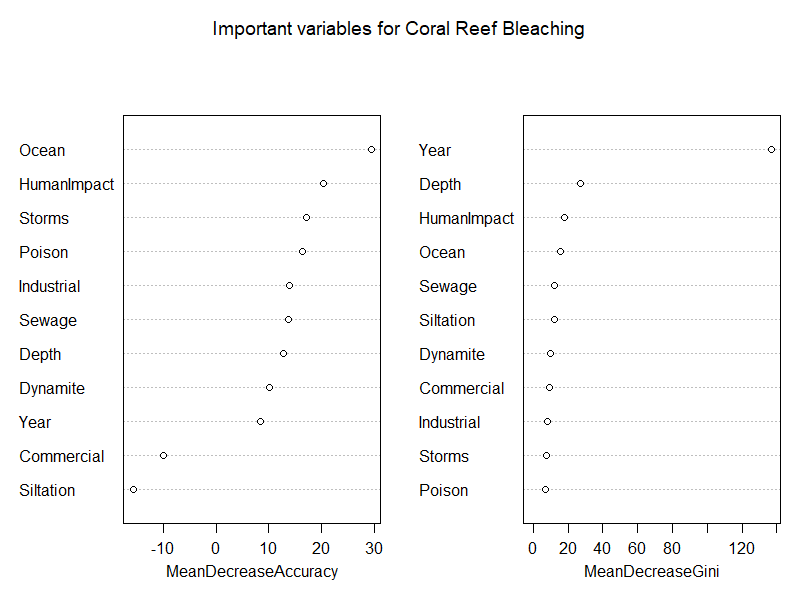
\includegraphics[scale=0.5]{/varImpPlot.png}
    \caption{Predictor Importance Plot for Coral Reef Bleaching (Unstandardized)}
    \label{vip}
\end{figure}
\newpage
Below, in Figure \ref{PP} we can see that the probability of no bleaching is much more likely as the year increases. This might be because of the possible errors in that variable, as I highlighted earlier. For the depth variable, we have an opposite effect. Lastly, unsurprisingly, for the human impact variable, we see that increasing from ``none'' to ``low'' increases the probability of bleaching, as we might expect, but this effect is smaller when the ``low'' type increases to the ``moderate'' or ``high'' category. 

\begin{figure}[!htb]
    \centering
    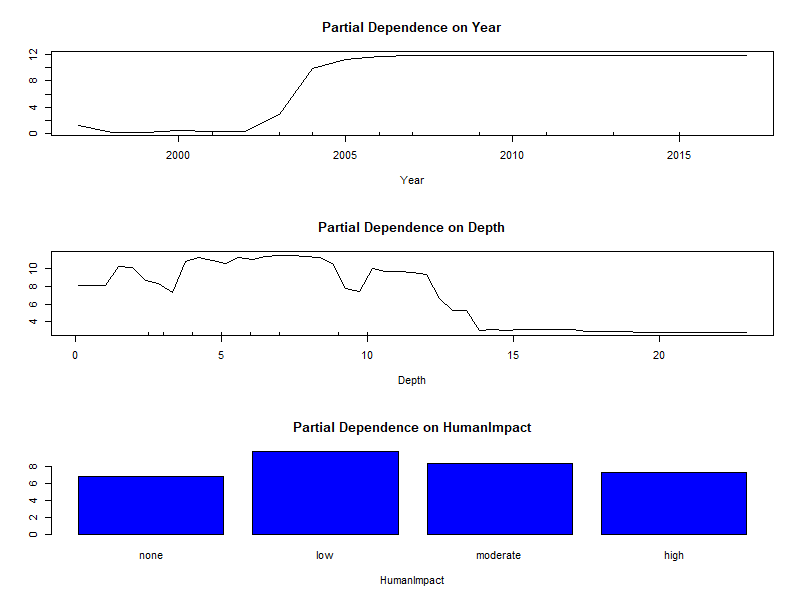
\includegraphics[scale=0.75]{/PartialPlots.png}
    \caption{Partial Dependence Plots for various variables on Bleaching.}
    \label{PP}
\end{figure}

\newpage

\section{Conclusion}
Based on the assumptions that I have made, the most important being the validity of the data\footnote{I think there could be some fair concerns raised about the strange behavior of the conditional distributions of the Year variable and the Commercial and Siltation variables.} and that the data is drawn from the appropriate joint probability distributions, the model results provide strong evidence that a random forest model would be a useful tool for policy makers to forecast which reefs would be at risk of bleaching, and thus require intervention. In particular, when moving beyond the OOB estimates to testing the trained model on the test dataset, I find that the errors are distributed in a manner very similar to the training model, and that the errors did not change significantly. This could alleviate one of the main concerns of implementing a random forest model ensemble, since this is some evidence that the over-fitting issue common in model ensemble algorithms might not be as present in this case. Without acquiring a stronger subject-matter knowledge and or more high quality data I believe it would be difficult to match this model's out-of-sample performance. Again, this result is still fairly tenuous, since without more subject-matter knowledge and confirmation of the quality of the data my result would not necessarily hold. 

\section{Appendix}
\begin{verbatim}
library(randomForest)
library(ggplot2)
library(xtable)
load("C:/Users/loren/Desktop/Machine Learning/Assignment 3/ReefCheck974.rdata")
#Renaming factors
levels(ReefCheck$Ocean)[levels(ReefCheck$Ocean) == ""] <-"unknown"
levels(ReefCheck$Storms)[levels(ReefCheck$Storms) == "none"] <-"unknown"
levels(ReefCheck$Storms)[levels(ReefCheck$Storms) == "y"] <-"yes"
levels(ReefCheck$HumanImpact)[levels(ReefCheck$HumanImpact) == ""] <-"none"
levels(ReefCheck$Storms)[levels(ReefCheck$Storms) == "unknown"] <-"no"
levels(ReefCheck$Siltation)[levels(ReefCheck$Siltation) == "unknown"] <-"never"
levels(ReefCheck$Siltation)[levels(ReefCheck$Siltation) == "Occasionally"] <-"occasionally"

levels(ReefCheck$Dynamite)[levels(ReefCheck$Dynamite) == ""] <-"none"
levels(ReefCheck$Poison)[levels(ReefCheck$Poison) == ""] <-"none"
levels(ReefCheck$Sewage)[levels(ReefCheck$Sewage) == ""] <-"none"
levels(ReefCheck$Sewage)[levels(ReefCheck$Sewage) == "k"] <-"moderate"

levels(ReefCheck$Industrial)[levels(ReefCheck$Industrial) == ""] <-"none"
levels(ReefCheck$Commercial)[levels(ReefCheck$Commercial) == ""] <-"none"

levels(ReefCheck$HumanImpact)[levels(ReefCheck$HumanImpact) == "unknown"] <-"none"
levels(ReefCheck$Poison)[levels(ReefCheck$Poison) == "unknown"] <-"none"

ReefCheck$Sewage = factor(ReefCheck$Sewage, levels = c("none", "low", "moderate", "high")) #Where applicable, I change the order to reflect the severity. 
ReefCheck$HumanImpact = factor(ReefCheck$HumanImpact, levels = c("none", "low", "moderate", "high"))
ReefCheck$Siltation = factor(ReefCheck$Siltation, levels = c("never", "occasionally", "often", "always"))
ReefCheck$Dynamite = factor(ReefCheck$Dynamite, levels = c("none", "prior", "low", "moderate", "high"))#why prior?
ReefCheck$Poison = factor(ReefCheck$Poison, levels = c("none", "low", "moderate", "high"))
ReefCheck$Industrial = factor(ReefCheck$Industrial, levels = c("none", "low", "moderate", "high"))
ReefCheck$Commercial = factor(ReefCheck$Commercial, levels = c("none", "low", "moderate", "high"))

save(ReefCheck, file ="CleanedReefCheck")

x = ReefCheck$Ocean[-which(ReefCheck$Ocean == "unknown")]
levels(x)[levels(x) == "unknown"] <- "Indian" #no unknown observations, can choose any level to drop it in to.
barplot(prop.table(table(x)), main = "Reef Location")


ggplot(ReefCheck, aes(Depth))+
  geom_histogram(col="grey", fill ="grey65", bins = 15)+
  theme(plot.title = element_text(hjust = 0.5))+
  labs(title="Depth of Reefs (meters)")

ggplot(ReefCheck, aes(Year))+
  geom_density(col="grey", fill ="grey65")+
  theme(plot.title = element_text(hjust = 0.5))+
  labs(title="Year of Reef Data Observations")

par(mfrow=c(2,2))
barplot(prop.table(table(ReefCheck$HumanImpact)), main = "Human Impact on Reefs")
barplot(prop.table(table(ReefCheck$Siltation)), main = "Siltation of Reefs" ) #why so often never?
barplot(prop.table(table(ReefCheck$Poison)), main = "Presence of Poison")
barplot(prop.table(table(ReefCheck$Sewage)), main = "Presence of Sewage") #why so often never?
par(mfrow=c(1,1))

#ReefCopy = ReefCheck
#ReefCopy$BleachingStorms = with(ReefCopy, interaction(ReefCopy$Bleaching, ReefCopy$Storms))
#ggplot(ReefCopy, aes(BleachingStorms))+ geom_bar(col="grey", fill ="grey65")+ theme(plot.title = element_text(hjust = 0.5))+  labs(title="Bleaching vs Storms")

#Bivariate analysis insight: Consider the conditional distribution of all independent variables, conditional on bleaching being true. 
#Are the statistics of independent variables of this conditional distribution different than when bleaching is false?
ReefNo = ReefCheck[which(ReefCheck$Bleaching == "No"),]
ReefYes = ReefCheck[which(ReefCheck$Bleaching == "Yes"),]

x1 = ReefYes$Ocean[-which(ReefCheck$Ocean == "unknown")]
levels(x1)[levels(x1) == "unknown"] <- "Indian"
x2 = ReefNo$Ocean[-which(ReefCheck$Ocean == "unknown")]
levels(x2)[levels(x2) == "unknown"] <- "Indian"

par(mfrow=c(2,1))
barplot(prop.table(table(x1)), main = "Location of Bleached Reefs")
barplot(prop.table(table(x2)), main = "Location of Healthy Reefs")
par(mfrow=c(1,1))


ggplot(ReefCheck, aes(Depth))+
  geom_density(col="grey", fill ="grey65")+
  facet_grid(Bleaching ~.)+
  theme(plot.title = element_text(hjust = 0.5))+
  labs(title="Depth of Reefs - Conditional on Reef Bleaching")

ggplot(ReefCheck, aes(Year))+
  geom_density(col="grey", fill ="grey65")+
  facet_grid(Bleaching ~.)+
  theme(plot.title = element_text(hjust = 0.5))+
  labs(title="Year of Reefs - Conditional on Reef Bleaching") #strange???

par(mfrow=c(3,4))
barplot(prop.table(table(ReefYes$Storms)), main = "Bleached-Storms") #no noticeable difference
barplot(prop.table(table(ReefNo$Storms)), main = "Healthy-Storms")
barplot(prop.table(table(ReefYes$HumanImpact)), main = "Bleached-HImpact") #in cases where there was higher levels of human impact, it's more likely to have had bleaching.
barplot(prop.table(table(ReefNo$HumanImpact)), main = "Healthy-HImpact")
barplot(prop.table(table(ReefYes$Siltation)), main = "Bleached-Silt") #very interesting! It seems that reefs that underwent bleaching never had siltation. No SM knowledge to understand this.
barplot(prop.table(table(ReefNo$Siltation)), main = "Healthy-Silt")
barplot(prop.table(table(ReefYes$Sewage)), main = "Bleached-Sewage") #Again, note that in the case of no sewage, bleaching is less likely.
barplot(prop.table(table(ReefNo$Sewage)), main = "Healthy-Sewage")
barplot(prop.table(table(ReefYes$Commercial)), main = "Bleached-Commerce") #interesting. Correlation between bleaching and no commercial activity near the reefs. 
barplot(prop.table(table(ReefNo$Commercial)), main = "Healthy-Commerce")
par(mfrow=c(1,1))




Index<-sample(1:12392, 9913, replace=FALSE)
Test <- ReefCheck[-Index,]
Train <- ReefCheck[Index,]
  

rf <- randomForest(Bleaching ~., data = Train, importance = T, sampsize = c(1150,187)) #Need to tweak the cost ratio.
print(rf)

rfPredict <- predict(rf, newdata = Test)
table(Test$Bleaching, rfPredict)

varImpPlot(rf,main="Important variables for Coral Reef Bleaching")
par(mfrow=c(3,1))
partialPlot(rf, Train, Year)
partialPlot(rf, Train, Depth)
#partialPlot(rf, Train, Ocean)
partialPlot(rf, Train, HumanImpact)
#partialPlot(rf, Train, Sewage)

\end{verbatim}


\end{document}
